\documentclass{article}
\usepackage[utf8]{inputenc}
\usepackage[margin=0.70in]{geometry}
\usepackage{graphicx} %插入图片的宏包
\usepackage{float} %设置图片浮动位置的宏包
\usepackage{subfigure} %插入多图时用子图显示的宏包

\title{Homework 2 (Part 1) Parallelizing a Particle Simulation}
\author{Andrew Chen, Brian Park, Xuan Jiang}
\date{February 2022}

\begin{document}

\maketitle
\section{Collaboration and Introduction}
Everyone on the team contributed equally. Xuan started off with implementation of particle binning to reduce the time complexity to $O(n)$. Brian was able to figure out an algorithmic way to speed up serial performance by reducing the number of comparisons per each iteration in a bin. Andrew was able to speed up Brian's implementation even more to a record time of 891 seconds (1000 particles) with a few more optimizations related to memory management. For OpenMP, Xuan and Brian was able to figure out how to add OpenMP directives to optimize code. Brian figured out how to parallelize for loops as adding locks and synchronization primitives to prevent false sharing, which hurt accuracy if done incorrectly. Everyone contributed equally to the report and everyone contributed to the group repository equally.

We used a variety of techniques to optimize the problem of parallelizing a particle simulation.
In the remainder of this report, we describe each of our optimizations in our final submission,
present results with evidence that they work, and describe attempted optimizations that did not
noticeably improve overall our performance.

\section{$O(N)$ time plots and description of data structures} 
\subsection{Plots}

\begin{figure}[H] %H为当前位置,!htb为忽略美学标准,htbp为浮动图形
\centering %图片居中
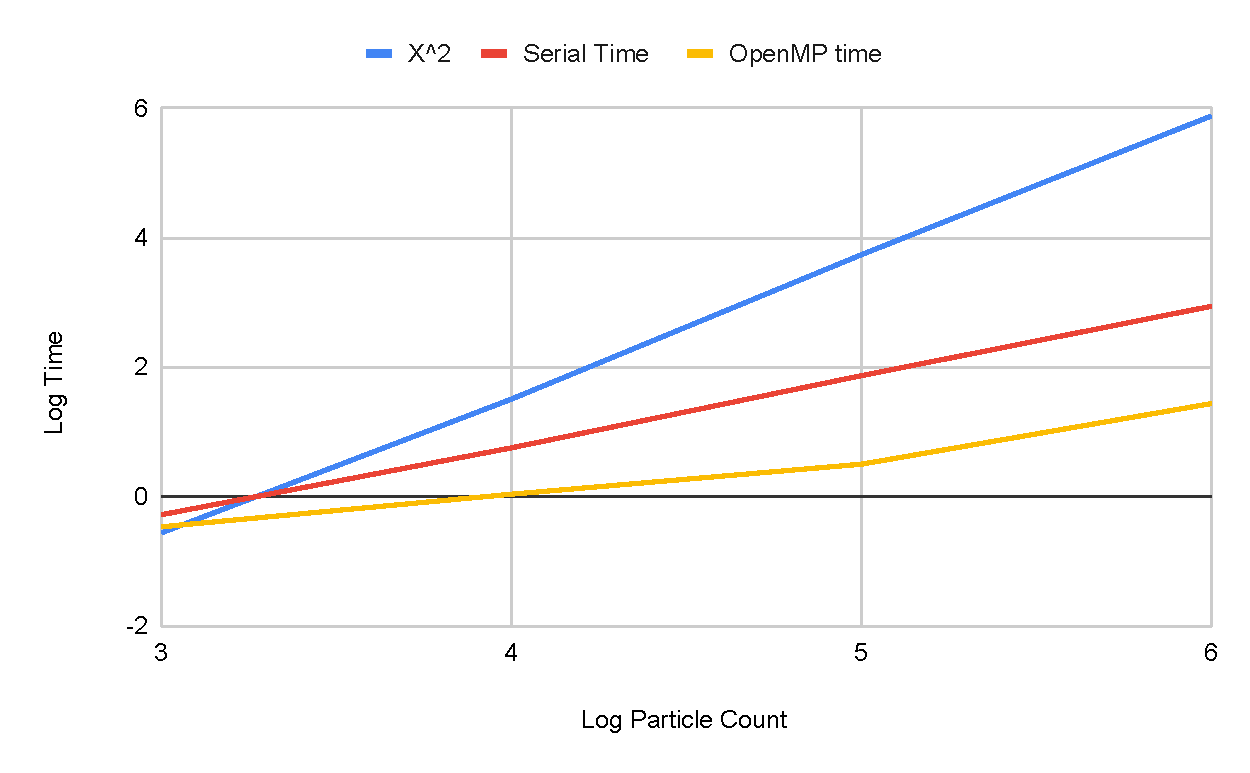
\includegraphics[width=0.7\textwidth]{log_plots.pdf} %插入图片,[]中设置图片大小,{}中是图片文件名
\caption{log-log scale showing plot time} %最终文档中希望显示的图片标题
\label{log-log scale showing plot time} %用于文内引用的标签
\end{figure}

As we can see from the Figure \ref{log-log scale showing plot time}, we have three plots of log-log sclae, where the blue one is the one with $O(n^{2})$ time complexity. And the red line represents for our serial optimization results. And the yellow line shows the results from our openmp implementation. And we have the particles vary from 1 thousand to 1 million to achieve the plot of Figure \ref{log-log scale showing plot time}. In our best scenario of serial implementation, we can compute the 1 million particles within 871.694 seconds. And in our openmp scenario, we further shrink the computation time to 26.7949 on 64 threads.

\subsection{Data Structures}
We defined our bins as vectors:

\verb|typedef vector<particle_t*> bin_t;|

\verb|bin_t* bins;|

We make sure that particles are stored in bins. The number of bins is fixed which is why we use an array of bins. The bins themselves
change in size each simulation as they move around, which is why we use \verb|std::vector|.
\section{Serial}

\subsection{Design Choice}
For the serial runtime code, we optimized the algorithm to be run $O(n^2)$ to $O(n)$. The way we cut down this runtime was by first doing particle binning. Since there is a threshold cutoff radius of how far two particles need to be to apply force on each other determined by \verb|r2 <= cutoff * cutoff|, we can partition the dataset into bins. That way, we can call \verb|apply_force| on a particle on it's neighboring bins, avoiding wasteful iterations on the whole dataset. We need to look in neighboring bins since the particle could lie on the edge of a bin and it could interact with a particle in a neighboring bin. First we optimized this by applying force and updating acceleration on eight neighboring bins of a particular bin, along with the bin itself. 
This brought us a speed of 2392.5 seconds for 1000 particles.

We can even do a further optimization and cut the number of total iterations by nearly half. We assume that we do a convolution of neighboring bins on each bin in row major order. Since force is applied and exerted on both particles, we can actually do two redundant computations at once. With that, that also requires a modification that only needs to compare four neighboring bins (right, lower left, lower, lower right). This brought our time even lower to 1629.9 seconds.

A similar optimization can be done when applying force to particles within one bin (ignoring neighboring bins). By applying force in pairs, and making sure to iterate over unique pairs of particles, iterations can be cut in half.

At this moment, our bins were represented by a 2d vector. However, we did not need the number of bins to be dynamic, and we switched our bins representation to be an array of vectors. This further brought the time
from 1629.9 to 1413.9 seconds.

In order to do the comparisons with the four neighboring bins mentioned earlier, we would check if it
was among nine possible location cases, and then calculate the valid locations of neighboring bins accordingly. We replaced these by having a loop which iterates over every possible coordinate of a neighboring bin, and checking if the coordinate is valid or not. This greatly simplifies the logic by replacing nine if statements with a loop and one if statement.

\begin{verbatim}
    for (int k = 0; k < bin.size(); k++) {
        for (auto& dir : dirs) {
            int xx = i + dir[0];
            int yy = j + dir[1];
            if (0 <= xx && xx < grid_size && 0 <= yy && yy < grid_size) {
                ...
\end{verbatim}

Interestingly, for 1000 particles, this brought the time up from 1413.9 seconds to 1544.6 seconds. Unfortunately,
the cost of the looping and coordinate validation is multiplied by the outer loop which iterates over particles within a bin. The series of nine if statements, although not as simple, essentially unrolls \verb|for (auto& dir : dirs)| and brings computation 
outside of the long outer loop. Thus, this logic change was not kept in the final version of our code.



Our implementation at this point also had inefficient memory management. For each \verb|simulate_one_step()|, we would set \verb|bins = new bin_t[grid_size * grid_size];| in order to clear out the bin vectors to prepare for the next simulation. Although
there are no loops, it turns out that this method of clearing all the vectors was slower than going through each vector and calling
\verb|vector.clear()| due to the overhead of deleting and re-mallocing a large array each simulation. Finally, the clearing of the bins
could be done immediately after applying the forces within the bin, so there did not need to be a dedicated
for loop for clearing. Combined with other small changes such as using the stack instead of the heap
where possible, passing by pointer instead of by value, time was reduced from 1413.9 seconds to 871s.


\section{OpenMP}
\subsection{Synchronization}
The first issue in parallelism with OpenMP was false sharing. Since multiple threads share the same main memory, false sharing could lead to inaccurate output. To circumvent this, OpenMP synchronization primitives are needed to make sure variables are thread-safe and not prone to false sharing. We used locks to protect data attributes via \verb|omp_set_lock| and \verb|omp_unset_lock|. Doing this will prevent any data races and false sharing. This also prevents deadlocks as we must acquire and release a lock. We believe that these are the minimal amount of synchronizations needed for protecting data, no need for conditional variables or semaphores. Alternatively, we could've done a reduction using an OpenMP directive, but for speeding it up purely based on our implementation of serial code, that would've required a lot of refactoring for the reduction and protection of data to work, thus we avoided it. We also needed to provide \verb|#pragma omp barrier| to synchronize between parallel sections. In conclusion, parallelization was easy as we explain in the next section, but synchronizing was the hardest part in order to product a correct output.

\subsection{Design Choice}
As OpenMP uses the fork join model, we had to make sure how to parallelize and minimize serialized code as much as possible. We tried to separate the code into several sections, and use \verb|#pragma omp master| for every section and change them one by one to \verb|#pragma omp for| to parallelize it. And then we implemented locks while updating bins, which is necessary since the \verb|std::vector| class is not thread safe in a multi-threaded context. We also need a \verb|#pragma omp barrier| before and after \verb|binning()| since we refresh the bins at each iteration. Although there is an implicit barrier after the end of every \verb|#pragma omp for|. This is because we need to refresh bins per every iteration, and \verb|simulate_one_step()| is already in a parallel context in \verb|main.cpp|. Barriers just ensure our data in bins is correct before and after the end of each iteration. Although adding more synchronization hurt our performance more, the trade off is necessary to prevent correction/floating point error. 

\subsection{Can We Do Better?}
Future possible optimizations include prefetching, and finding a smaller bin size to use. This is to exploit cache locality since a thread/core will share L1 and L2 cache. Lower levels of the memory hierarchy like L3 and main memory are shared amongst cores. If we wanted, we could also exploit DLP (data level parallelism) with the use of SIMD. This type of optimization is much harder to do since we're working with classes and data is not necessary tightly packed and DLP friendly like the data in our matrix multiplication homework. Compared the the TLP (thread level parallelism) that KNL node provides (68 cores/ 272 threads), it's a much easier optimization to achieve speedup with purely MIMD. Finally, it's possible we used more synchronization than necessary for correctness. For instance, a few barriers and locks
could possibly be removed if done correctly.

\section{Speed up plots and discussion}
\subsection{Weak Scaling}
\begin{figure}[H] %H为当前位置,!htb为忽略美学标准,htbp为浮动图形
\centering %图片居中
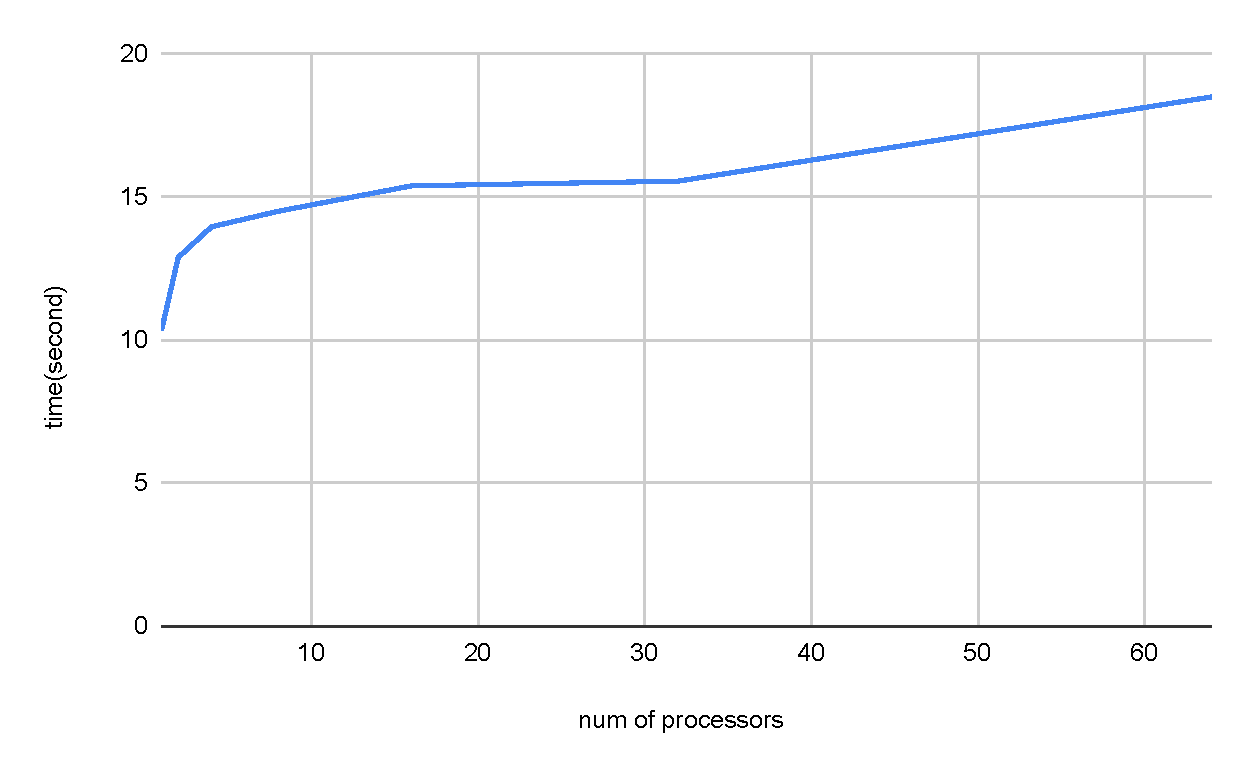
\includegraphics[width=0.7\textwidth]{time_vs_num_processor_weak.pdf} %插入图片,[]中设置图片大小,{}中是图片文件名
\caption{Time VS number of Processors} %最终文档中希望显示的图片标题
\label{Time VS number of Processors} %用于文内引用的标签
\end{figure}

We are only seeing a little jump on from 1 processor to 2 processors and then we are remaining good performance on increasing number of processors by two times.


\begin{figure}[H] %H为当前位置,!htb为忽略美学标准,htbp为浮动图形
\centering %图片居中
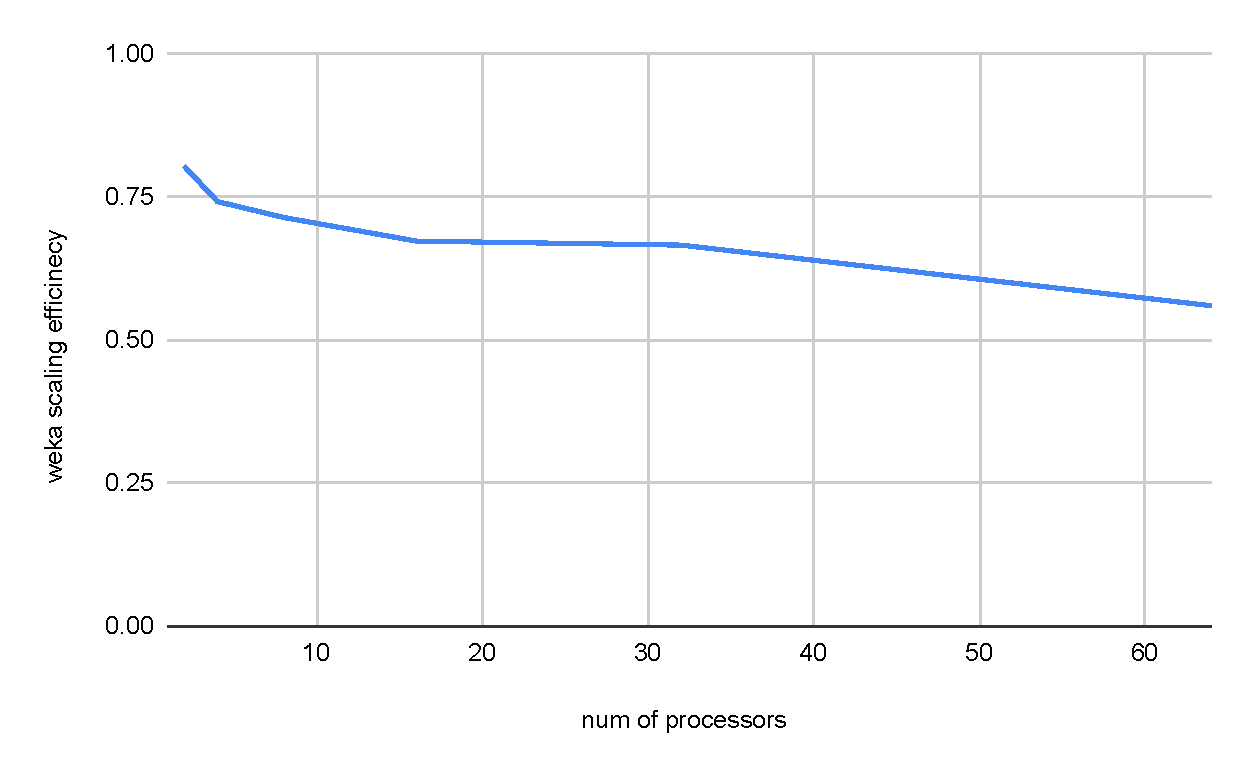
\includegraphics[width=0.7\textwidth]{weka scaling efficinecy vs. num of processors.pdf} %插入图片,[]中设置图片大小,{}中是图片文件名
\caption{Weak Scaling Efficiency vs number of processors} %最终文档中希望显示的图片标题
\label{Weak Scaling Efficiency vs number of processors} %用于文内引用的标签
\end{figure}

We can see that our weak scaling efficiency is highest while we are using 2 processor which is 88.27\% and when we increasing the number of of processors and number of particles by the same times, the weak scaling efficiency is going all the way down to 55.92\%, but it's still pretty good.

\subsection{Strong Scaling}

We fixed our problem size to be 1 million particles and keep on increasing the number of processors from 1 all the way to 64 by 2 times every time, and the following shows the computation time changes
\begin{figure}[H] %H为当前位置,!htb为忽略美学标准,htbp为浮动图形
\centering %图片居中
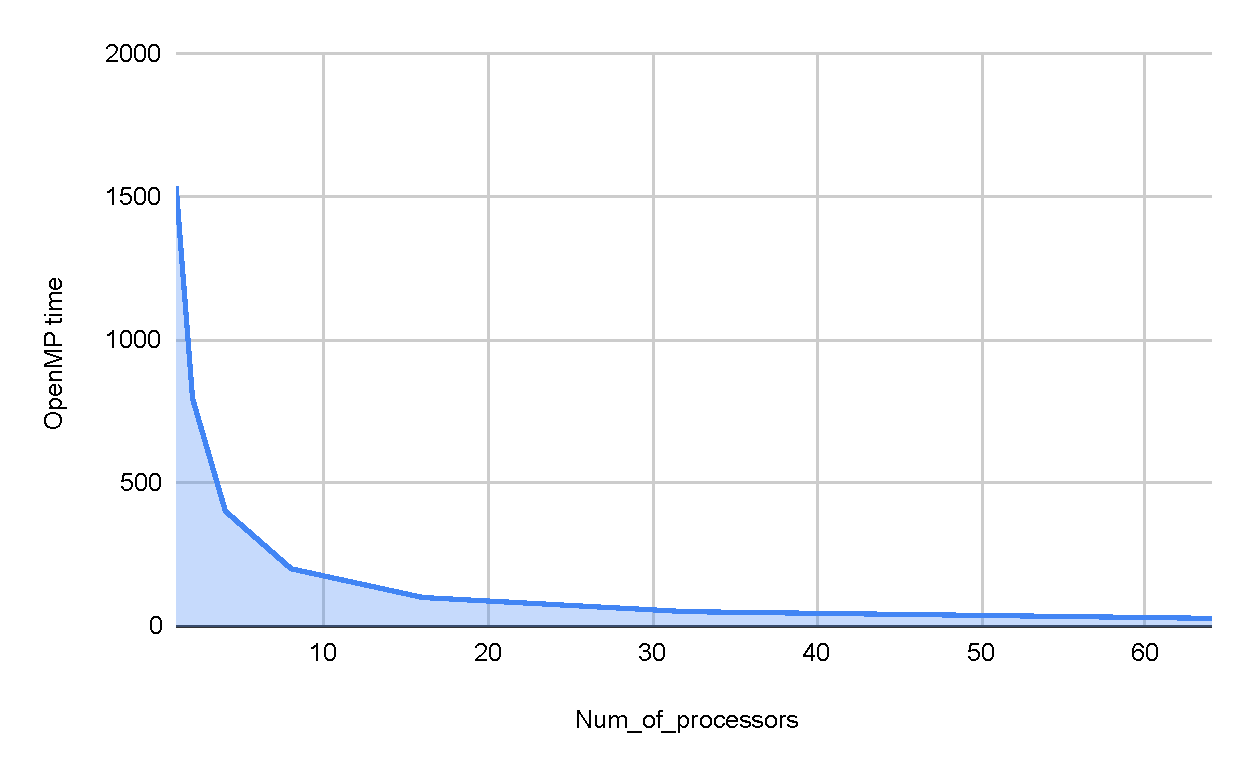
\includegraphics[width=0.7\textwidth]{OpenMP time vs. Num_of_processors_strong.pdf} %插入图片,[]中设置图片大小,{}中是图片文件名
\caption{Time VS Number of Processors} %最终文档中希望显示的图片标题
\label{Time VS Number of Processors} %用于文内引用的标签
\end{figure}

We can see that with the changes from 1 processor to 2 processors our total time shrinks almost by half, and we are maintaining the high performance in the following parts with keeping increasing of processors.

\begin{figure}[H] %H为当前位置,!htb为忽略美学标准,htbp为浮动图形
\centering %图片居中
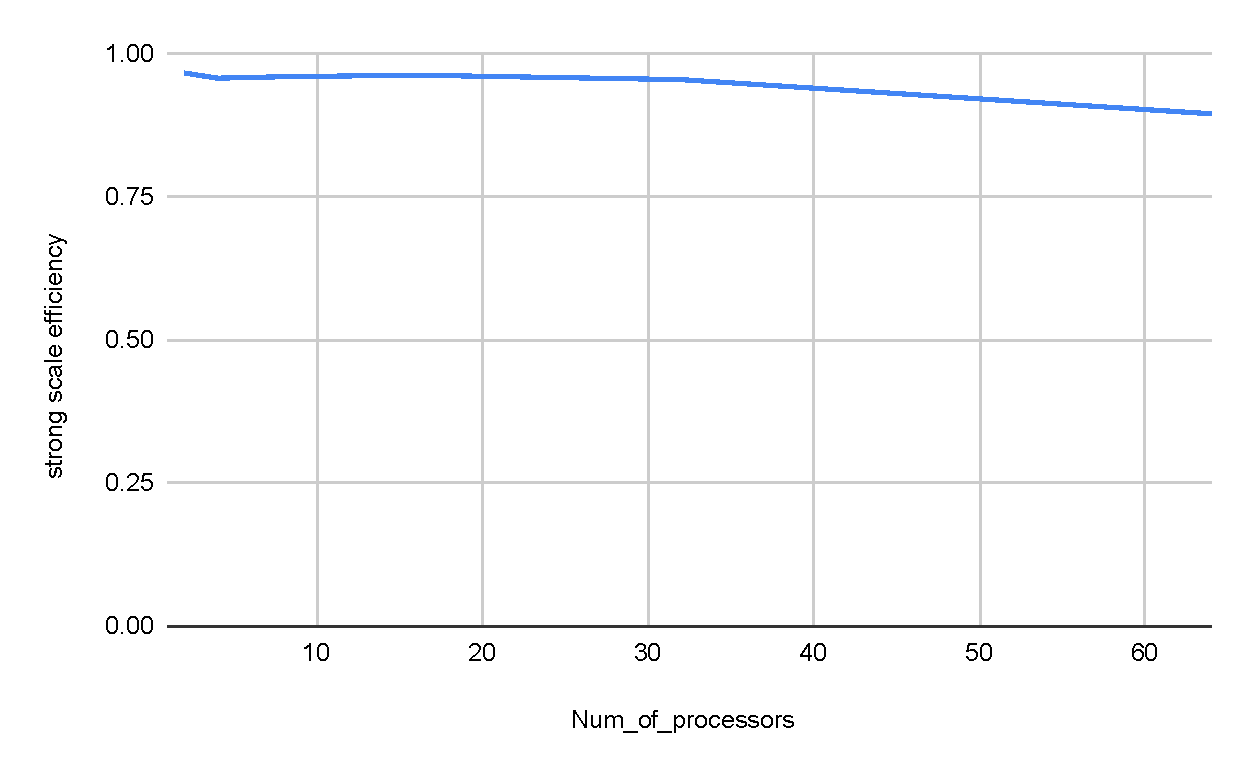
\includegraphics[width=0.7\textwidth]{strong scale efficiency vs. Num_of_processors.pdf} %插入图片,[]中设置图片大小,{}中是图片文件名
\caption{Strong Scaling Efficiency VS Num of processors} %最终文档中希望显示的图片标题
\label{Strong Scaling Efficiency VS Num of processors} %用于文内引用的标签
\end{figure}

We can see from the picture that we are having 96.56\% strong scaling efficiency when we increased our processor from 1 to 2. And it's almost always be around 95\% strong scaling efficiency. And we finally achieve a 89.44\% strong scaling efficiency after we increase our number of processors to 64.
\subsection{Whether It's Possible To Do Better.}


We think we will be able to improve the $p$-times speedup by removing synchronization, because the synchronization will cause a significant amount of usage of time based on our time break downs below. And It will help, because synchronization stalls code to enter critical section.

But this is in theory, if we want to remove the synchronization we will need to refactor the whole implementation. Because the usage of vectors is why we must need synchronization, because vector class is not thread safe in a parallel context.

And another part we can improve is that we are using so many locks than necessary which is draging down the speed as well.

And we further discuss what we can do better in section 4.3



\section{Performance Breakdown}
For this no communication time was recorded, as we are purely working with a shared memory system. Below is the times we see when timing computation times and synchronization times. For computation, we left the code without any explicit barriers, and for synchronization, we left barriers on. We see that they have nearly the same times. We used print statements as we didn't really know how to utilize the profiling tools, the learning curve for using it was very steep.

\begin{figure}[H] %H为当前位置,!htb为忽略美学标准,htbp为浮动图形
\centering %图片居中
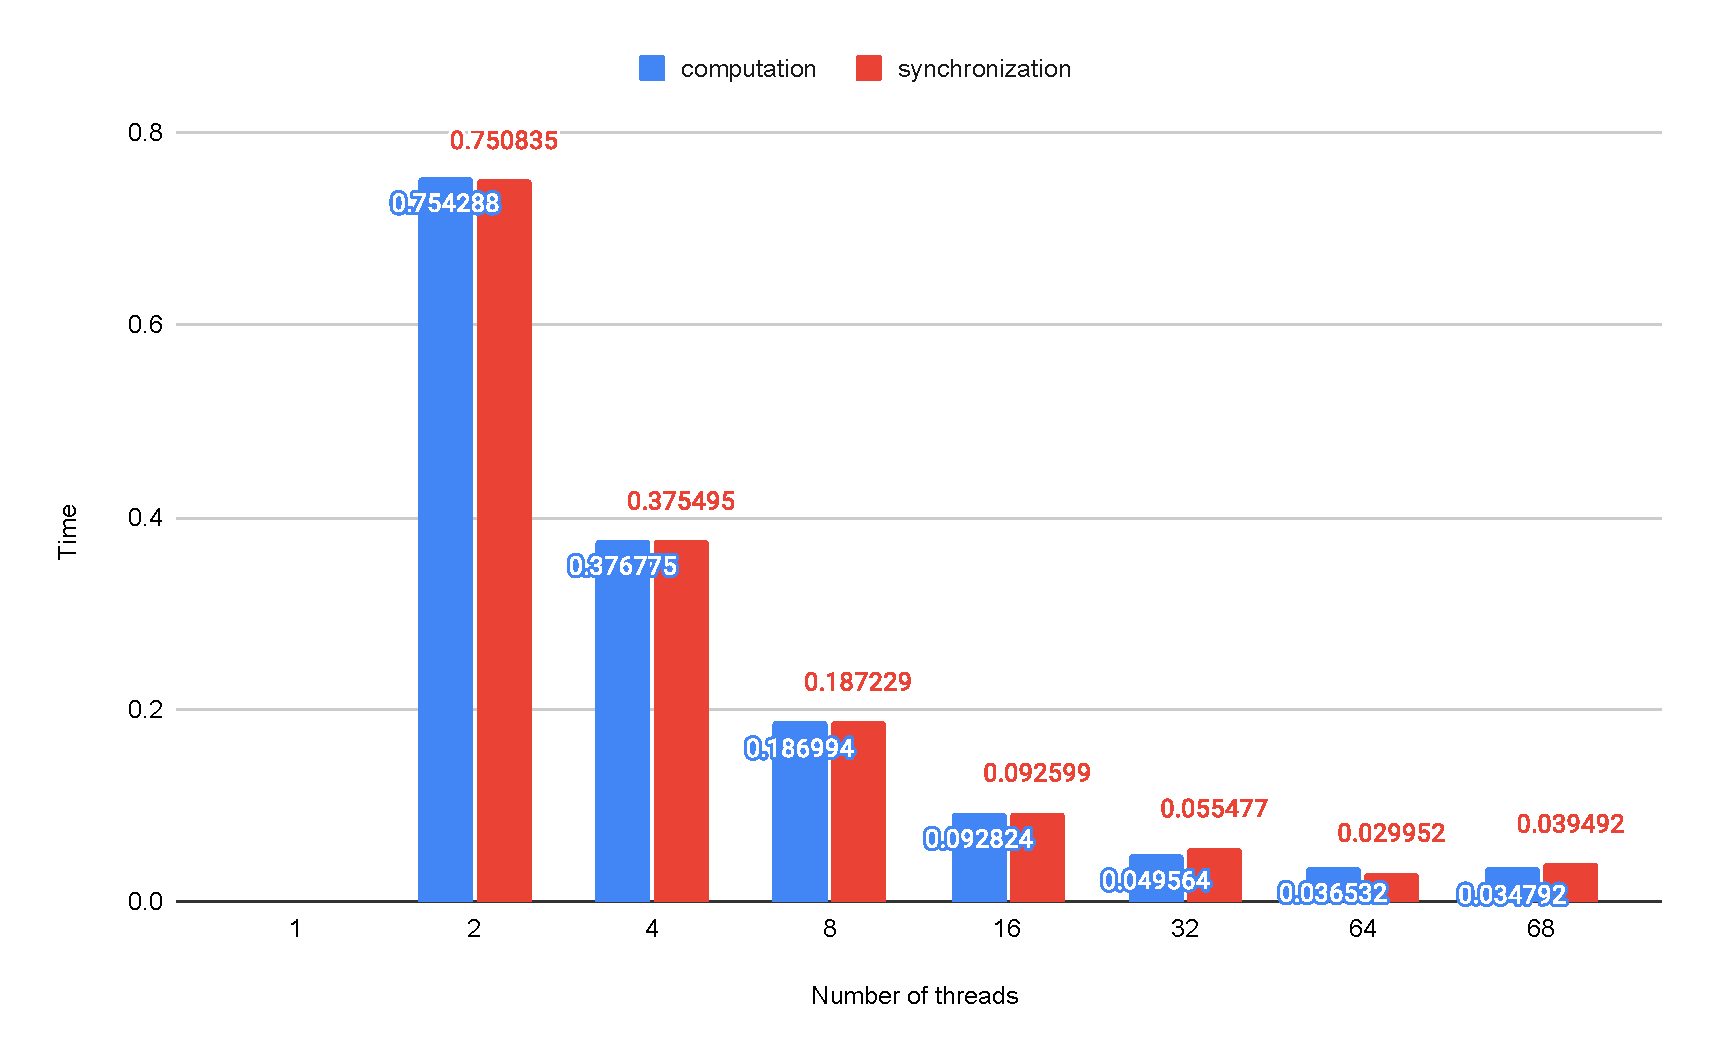
\includegraphics[width=0.7\textwidth]{time_break_down.pdf} %插入图片,[]中设置图片大小,{}中是图片文件名
\caption{Time break downs with the scale of p changes} %最终文档中希望显示的图片标题
\label{Strong Scaling Efficiency VS Num of processors} %用于文内引用的标签
\end{figure}







% Write-up Details

% Your write-up should contain:

% The names of the people in your group and each member's contribution.

% A plot in log-log scale that shows that your serial and parallel codes run in O(n) time and a description of the data structures that you used to achieve it.

% A description of the synchronization you used in the shared memory implementation.

% A description of the design choices that you tried and how did they affect the performance.

% Speedup plots that show how closely your OpenMP code approaches the idealized p-times speedup and a discussion on whether it is possible to do better.

% Where does the time go? Consider breaking down the runtime into computation time, synchronization time and/or communication time. How do they scale with p?

% Notes:

% Your grade will mostly depend on three factors:

% Scaling sustained by your codes on the Cori supercomputer (varying n).

% Performance sustained by your codes on the Cori supercomputer.

% Explanations of your methodologies and the performance features you observed (including what didn't work).

% You must use the GNU C Compiler for this assignment. If your code does not compile and run with GCC, it will not be graded.

% If your code produces incorrect results, it will not be graded.

% You must target Cori's KNL processors for this assignment, not Haswell, like HW1.

\end{document}
